\subsection{Example: Decomposing \texttt{sub}}

Consider the 32-bit integer \tt{0x00012122}. In this example, we will
parse the number in a sequence of steps, before finally arriving at
that this number represents an instance of the \tt{sub} instruction.

In an earlier section we established the input and output of our
decompiler, see Fig.~\eqref{fig:mips32-decompiler} which maps nicely
into Table.~\ref{table:instruction-operations}. In this example we
will start by supplying our factory
method \mij{Instruction.fromInteger(int instruction)} with
\tt{0x00012122}

\begin{figure}[H]
  \centering 
  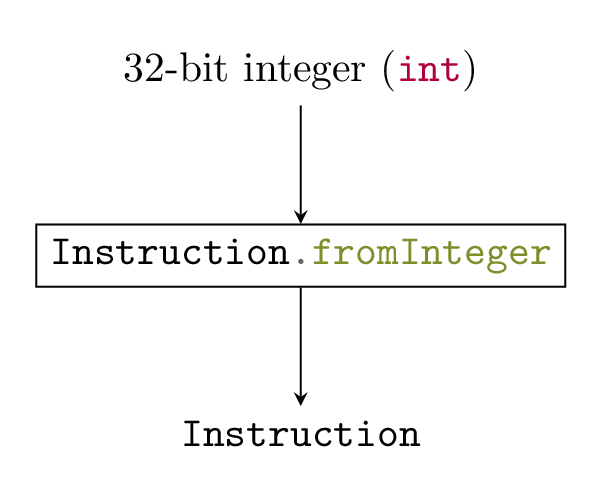
\includegraphics[width=0.7\textwidth]{figures/mips32-decompiler-interface.png} 
  \caption{Interface} \label{fig:mips32-decompiler-interface}
\end{figure}

and get an object \mij{Instruction} capable of representing itself.

\subsubsection{Determining \texttt{Opcode} from a 32-bit integer}
First, we have that the \tt{Opcode} may be determined by the 6
left-most bits of the number, hence we would like to have a function
$f$ such that,

\begin{equation*}
f: \textrm{32-bit integer} \to \tt{Opcode}
\end{equation*}

In Java we can represent this by having a class, \opcodem\footnote{
\tt{src/main/java/se.filipallberg.dark.mips32decompiler.instruction.util.Opcode}}
with the method,

\begin{minted}{java}
public static Opcode fromInstruction(int instruction);
\end{minted}

The \opcodem abstraction will intermittently be represented in
numerical form, so in this
case \mintinline{java}{Opcode.fromInstruction(0x00012122)} will
occassionally be written out as \tt{0x00}. The class, \opcodem,
supplies handy utility methods for representing itself either as an
object or the \mij{int} primitive.


\subsubsection{Mnemonic patterns}


\subsection{An decompilation algorithm}

Using the functions expressed in the previous sections we are now ready to
define an algorithm for our 32-bit integers.

\LetLtxMacro\i\textit
\newcommand{\get}[2]{\tt{#1} \i{#2} $\gets$ }
\newcommand{\of}[1]{(\i{#1})}
\newcommand{\from}[1]{\i{#1}}

\begin{algorithm}
\caption{Parsing/Decompilation algorithm}\label{algo:decompile}
\begin{algorithmic}[1]
\Procedure{Parse}{32-bit integer \i{int}}
\State \get{Opcode}{o}\from{getOpcode}\of{int}
\State \get{Format}{format}\from{getFormat}\of{o}
\State \get{InstructionName}{iname}\from{getName}\of{format, int}
\State \tt{DecomposedRepresentation} d
\State \get{}{d}\from{getDecomposedRepresentation}\of{format, int}
\State \get{String}{dec}\from{decimal}\of{d}
\State \get{String}{hex}\from{hex}\of{d}
\State \get{MnemonicPattern}{r}\from{getMnemonicPattern}\of{iname}
\State \tt{MnemonicRepresentation} mnemonic
\State \get{}{mnemonic}\from{getMnemonicRepresentation}\of{iname, r, d} \\
\Return (int, format, dec, hex, mnemonic)
\EndProcedure
\end{algorithmic}
\end{algorithm}



